\chapter{Reflectie en discussie}
\label{discH}
In dit laatste hoofdstuk zullen we een analyse maken van het praktische deel van ons project.
We beginnen met een discussie van de gebruikte methoden en bruikbaarheid van de gevonden resultaten.
Verder worden de resultaten besproken voor het comprimeren van afbeeldingen, het toepassen van het 
Tensorproduct en als laatste het gebruik van de Tensor/Mallat mengvorm op filmmateriaal. 

\section{Discussie}
\subsection{Gebruik van PSNR als maatstaf voor kwaliteit}
Omdat we te maken hebben met `lossy' beeldcompressie dienen we dit verlies in kaart te brengen op een 
objectieve en kwantitatieve manier. 
De PSNR is een gebruikelijke grootheid voor dit soort analyses, er wordt gezegd dat dit voor eenzelfde 
beginsignaal een goede reflectie geeft van de menselijke beleving van de kwaliteit van de reconstructie.
Uit onderzoek\cite{PSNR} blijkt dat de PSNR een goede maatstaf is zolang er in zeker zin \emph{ceteris paribus}
is aangehouden; voor hetzelfde beeldmateriaal presteert het goed.

\subsection{Bruikbaarheid van resultaten}

De resultaten beslaan slechts een kleine set beelmateriaal, dit heeft vooral met tijdgebrek te maken gehad.
We zullen geen uitspraak doen over een bepaalde beelcategorie (zoals boven beschreven) omdat hier simpelweg te
weinig studie naar is verricht, echter menen we dat de set beelden gevari\"eerd genoeg is om algemene uitspraken te doen
over de prestatie van de verschillende algoritmes.

\section{Fourier/Wavelet compressie van afbeeldingen}

\subsection{Prestatie van Fourier vs. Wavelets}
Uit de PSNR grafieken blijkt dat de Fouriertransformatie een slechtere reconstructie levert voor dezelfde dataset
dan zowel de Haar als de Daubechies(2/4) wavelettransformaties, ongeacht de catagorie waartoe het beeld behoort.

\subsection{Wavelet vs. Wavelet}
Tussen de twee wavelets zien we verder wat we theoretisch verwachten, Haar presteert goed bij harde randen en grote kleurvlakken
vanwege zijn kleine drager, terwijl Daubechies voor fotografisch materiaal een goede reconstructie geeft door zijn grote drager.
We kunnen dit echter niet hard maken doordat we te weinig beeldmateriaal hebben bekeken in de verschillende catagori\"een. 

\subsection{Convergentie bij kleine dataset}
Uit de grafiek blijkt dat het verschil in kwaliteit tussen de verschillende compressie algoritmes afneemt wanneer
de hoeveelheid data die opgeslagen wordt klein wordt. 
Door de kleine dataset is de willekeur van de vorm van het plaatje erg van invloed op kwaliteit van de reconstructie 
voor verschillende algoritmes. 
Ook is het dubieus of de PSNR nog een goede maatstaf is voor de menselijke perceptie wanneer de algoritmes
zo'n slechte maar zeer verschillende benadering geven van het originele beeld.
We zullen daarom hier geen uitspraak over kunnen doen.

\section{Het Tensorproduct op afbeeldingen}
Voor de volledigheid hebben we er voor gekozen \'o\'ok het Tensorproduct te bekijken bij een aantal van onze afbeeldingen: zie figuren \ref{fig:tensor_start}-\ref{fig:tensor_end}. We hebben er voor gekozen om niet alle afbeeldingen in dit formaat weer te geven omdat de strekking wel duidelijk wordt uit een tweetal.

Het eerste wat op te merken valt, zijn de horizontale en verticale balken die bij het Tensorproduct ineens tevoorschijn komen. Deze zijn in de Mallatdecompositie een stuk minder aanwezig. De reden hiervoor is redelijk simpel aan te wijzen. Bij de Mallatdecompositie bekijken we wavelets met een drager die in beide richtingen even groot is (een vierkant dus). Het Tensorproduct legt deze eis natuurlijk niet op met als gevolg dat er een wavelet is met een drager die heel breed is en ook weer heel kort: een balk dus. Als deze balk door de compressie-algoritme weggelaten wordt, mist de reconstructie hier een benadering en kan er een gekke horizontale balk in de reconstructie onstaan.

Het tweede wat we opmerkten is dat de PSNR structureel lager is bij het Tensorproduct in vergelijking met de Mallatdecompositie. Dit komt ook wel overeen met wat we zien in de figuren \ref{fig:tensor_start} en \ref{fig:tensor_end}. Merk wel op dat vooral figuur \ref{fig:tensor_start} een extreem voorbeeld is en dat de verschillen in figuur \ref{fig:tensor_end} al een stuk minder overheersend zijn.

Het is interessant om op te merken dat onze metingen -- dat het Tensorproduct consistent lagere PSNR-waardes oplevert -- in strijd zijn met de claims die gemaakt worden in \cite{tensor_vs_mallat}, hoewel er teveel onbekende factoren zijn om te weten of dit misschien een andere reden heeft.
\section{Gemenge decompositie op 3D signalen}
Hoewel het bekijken van 3D signalen in ons project een leuke toevoeging was, is de analyse wat moeilijker gebleken. Dit heeft eigenlijk twee redenen.

Ten eerste is onze implementatie, hoewel misschien effici\"ent, niet erg snel. Het comprimeren van een afbeelding duurt ongeveer dertig seconden en het comprimeren van een filmpje duurt al snel het vijftigvoudige. Als gevolg hiervan wordt het comprimeren van meerdere 3D signalen een langdurige taak.

Daarnaast hebben we veel moeite gehad om passend beeldmateriaal te vinden. Uit het eerste punt volgt dat dit beeldmateriaal klein in afmetingen moet zijn en er moet wel wat gebeuren. Dit maakte de zoektocht lastig.

\subsection{PSNR}
Hoewel de PSNR in het geval van de afbeeldingen een prima representatie geeft van hoe goed de reconstructie op het originele signaal lijkt, blijkt het bij het beeldmateriaal dat wij bekeken hebben minder goed te werken. Zie figuur \ref{fig:cockto}. We hebben dan ook besloten hier geen aandacht aan te besteden.

\begin{figure}[h]
\centering
\begin{subfigure}[t]{0.48\textwidth}
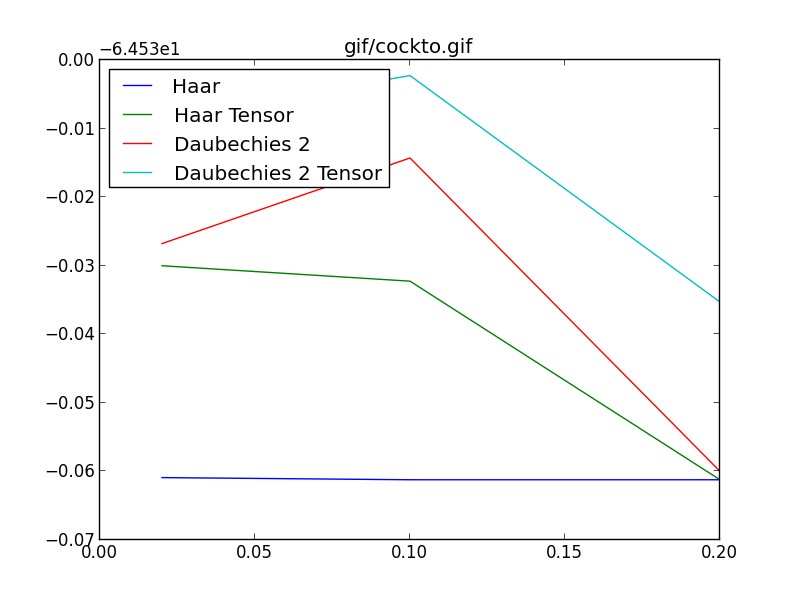
\includegraphics[width=\linewidth]{plaatjes/cockto.png}
\end{subfigure}
\begin{subfigure}[t]{0.48\textwidth}
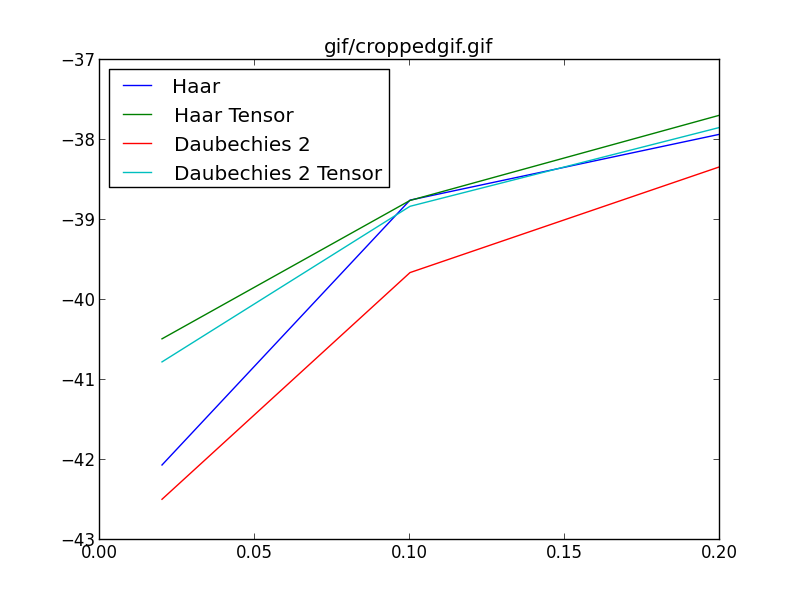
\includegraphics[width=\linewidth]{plaatjes/croppedgif.png}
\end{subfigure}
\caption{Links: de grafiek horende bij de dansende octopus. Rechts: de grafiek horende bij de scene met de typmachine en de boom.}
\label{fig:cockto}
\end{figure}

\subsection{Mallatdecompositie versus de mengvorm}
Wat we wel direct opmerkten is het enorme verschil in detail tussen de twee compressiemethoden. Dit komt omdat het Tensorproduct sneller convergeert bij continue signalen (zie stellingen \ref{thm:foutmallat} en \ref{thm:fouttensor}). Omdat een bewegend beeld over het algemeen continu is in de tijdsdimensie, is het gevolg niet vreemd.

Wanneer er w\'el een grote sprong in de tijd optreedt, zoals bij een scenewisseling, is de fout van het Tensorproduct ineens een stuk groter dan die van de Mallatdecompositie. Dit is vooral duidelijk bij de typmachinescene. Het gele mannetje verdwijnt bij de Mallatdecompositie na ongeveer 5 tijdseenheden waarbij hij bij het Tensorproduct na 8 frames nog steeds zichtbaar is.

TODO: Hier moeten we gewoon wat stills gebruiken in plaats van vage naamgeving.


